\section{The board the winners were playing}
\label{sec:board}

Table~\ref{tab:board} lists the final top ten together with their public standing.
The private board reordered almost everything: the winner was seventh on public, the
third-place team eleventh, the fourth fourteenth, while the public leader was not in the
private top 200 at all.

\begin{table}[t]
\centering
\small
\caption{Final private leaderboard (top ten) with the same teams' public standing.
``Public'' is the best public submission each team recorded, so a team can appear higher
there than the file that produced its private score. Team 10 and 11 tie at five decimals.}
\label{tab:board}
\begin{tabular}{rlrrrl}
\toprule
\# & Team & public rank & public \auc{} & private \auc{} & public write-up\\
\midrule
1  & Chris Deotte              & 7   & 0.96261 & 0.96318 & yes \citep{kaggle_first}\\
2  & Prior (3 members)         & 9   & 0.96252 & 0.96308 & no\\
3  & Christoffer Thimsen       & 11  & 0.96241 & 0.96306 & no\\
4  & Ole-Jakob                 & 14  & 0.96236 & 0.96304 & yes \citep{kaggle_fourth}\\
5  & Abdelrahman mohsen        & 10  & 0.96242 & 0.96292 & yes (short) \citep{kaggle_fifth}\\
6  & srikalyan                 & 12  & 0.96238 & 0.96280 & no\\
7  & UIT --- Loc \& An         & 403 & 0.96213 & 0.96263 & yes \citep{kaggle_seventh}\\
8  & Maher el Ouahabi          & 541 & 0.96199 & 0.96262 & no\\
9  & Fritz Cremer              & 8   & 0.96260 & 0.96259 & yes \citep{kaggle_ninth}\\
10 & Vivillon                  & 37  & 0.96226 & 0.96254 & no\\
\midrule
--- & this repository (8-family blend) & 1{,}204 & 0.96062 & 0.96133 & ---\\
\bottomrule
\end{tabular}
\end{table}

\subsection{The public board was a different game}

Figure~\ref{fig:lb} (left) plots public against private score for the 200 teams whose
private score we can see. Three facts stand out.

\emph{The public top five mostly vanished.} Public scores above 0.963 were achieved by five
teams; four of them (0.96473, 0.96451, 0.96375, 0.96319) do not appear in the private top
200, and the fifth fell to 58th (0.96239). The public board is 30\% of the test set, so it
is noisier than the private one --- but only by about $\sqrt{70/30}\approx1.5$ in standard
error. That cannot explain a $10^{-3}$ gap; fitting the 30\% can.

\emph{Everyone else moved up, by the same amount.} 99\% of the private top 200 scored
higher on private than on public, with a mean shift of \dlt{4.2}
(Figure~\ref{fig:lb}, right). Our submission shows the same constant offset
(0.96062 $\to$ 0.96133, \dlt{7.1}). The offset is a property of the split, not of a team.

\emph{Above 0.9623 the board is a tie.} The private scores from rank 75 onward are all
0.96238: 126 of the first 200 rows share that value. That is not 126 independent
discoveries; it is the same column of public OOF predictions stacked with slightly
different code and submitted at the same granularity. The cheap part of this competition
was over long before the deadline.

The consequence for reading the rest of this document: differences of \dlt{1} among the
top teams are mostly selection noise, while differences of \dlt{5} and more are structural.
The two grammars below differ by more than that.

\begin{figure}[t]
\centering
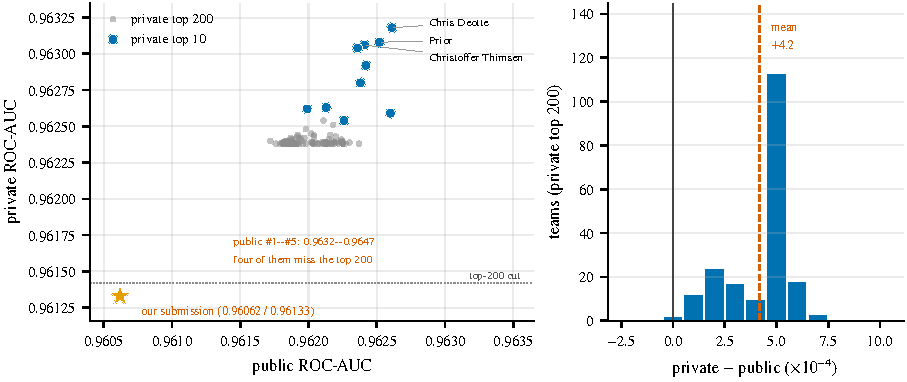
\includegraphics[width=\linewidth]{figures/fig_lb.pdf}
\caption{Left: public versus private score for the 200 teams whose private score is
visible. The top four public entries are off this axis to the right; four of the public
top five are absent from the private top 200. Right: distribution of the private$-$public
difference for the same teams (mean \dlt{+4.2}). The horizontal band of grey points on the
left is the 0.96238 tie. Our submission is marked for scale.}
\label{fig:lb}
\end{figure}
